\documentclass[11pt]{article}

    \usepackage[breakable]{tcolorbox}
    \usepackage{parskip} % Stop auto-indenting (to mimic markdown behaviour)
    \usepackage{xeCJK} 
    \usepackage{fontspec, xunicode, xltxtra}
    \setCJKmainfont{思源宋體}
    \XeTeXlinebreaklocale "zh" 
    \XeTeXlinebreakskip = 0pt plus 1pt 

    \usepackage{iftex}
    \ifPDFTeX
    	\usepackage[T1]{fontenc}
    	\usepackage{mathpazo}
    \else
    	\usepackage{fontspec}
    \fi

    % Basic figure setup, for now with no caption control since it's done
    % automatically by Pandoc (which extracts ![](path) syntax from Markdown).
    \usepackage{graphicx}
    % Maintain compatibility with old templates. Remove in nbconvert 6.0
    \let\Oldincludegraphics\includegraphics
    % Ensure that by default, figures have no caption (until we provide a
    % proper Figure object with a Caption API and a way to capture that
    % in the conversion process - todo).
    \usepackage{caption}
    \DeclareCaptionFormat{nocaption}{}
    \captionsetup{format=nocaption,aboveskip=0pt,belowskip=0pt}

    \usepackage[Export]{adjustbox} % Used to constrain images to a maximum size
    \adjustboxset{max size={0.9\linewidth}{0.9\paperheight}}
    \usepackage{float}
    \floatplacement{figure}{H} % forces figures to be placed at the correct location
    \usepackage{xcolor} % Allow colors to be defined
    \usepackage{enumerate} % Needed for markdown enumerations to work
    \usepackage{geometry} % Used to adjust the document margins
    \usepackage{amsmath} % Equations
    \usepackage{amssymb} % Equations
    \usepackage{textcomp} % defines textquotesingle
    % Hack from http://tex.stackexchange.com/a/47451/13684:
    \AtBeginDocument{%
        \def\PYZsq{\textquotesingle}% Upright quotes in Pygmentized code
    }
    \usepackage{upquote} % Upright quotes for verbatim code
    \usepackage{eurosym} % defines \euro
    \usepackage[mathletters]{ucs} % Extended unicode (utf-8) support
    \usepackage{fancyvrb} % verbatim replacement that allows latex
    \usepackage{grffile} % extends the file name processing of package graphics 
                         % to support a larger range
    \makeatletter % fix for grffile with XeLaTeX
    \def\Gread@@xetex#1{%
      \IfFileExists{"\Gin@base".bb}%
      {\Gread@eps{\Gin@base.bb}}%
      {\Gread@@xetex@aux#1}%
    }
    \makeatother

    % The hyperref package gives us a pdf with properly built
    % internal navigation ('pdf bookmarks' for the table of contents,
    % internal cross-reference links, web links for URLs, etc.)
    \usepackage{hyperref}
    % The default LaTeX title has an obnoxious amount of whitespace. By default,
    % titling removes some of it. It also provides customization options.
    \usepackage{titling}
    \usepackage{longtable} % longtable support required by pandoc >1.10
    \usepackage{booktabs}  % table support for pandoc > 1.12.2
    \usepackage[inline]{enumitem} % IRkernel/repr support (it uses the enumerate* environment)
    \usepackage[normalem]{ulem} % ulem is needed to support strikethroughs (\sout)
                                % normalem makes italics be italics, not underlines
    \usepackage{mathrsfs}
    

    
    % Colors for the hyperref package
    \definecolor{urlcolor}{rgb}{0,.145,.698}
    \definecolor{linkcolor}{rgb}{.71,0.21,0.01}
    \definecolor{citecolor}{rgb}{.12,.54,.11}

    % ANSI colors
    \definecolor{ansi-black}{HTML}{3E424D}
    \definecolor{ansi-black-intense}{HTML}{282C36}
    \definecolor{ansi-red}{HTML}{E75C58}
    \definecolor{ansi-red-intense}{HTML}{B22B31}
    \definecolor{ansi-green}{HTML}{00A250}
    \definecolor{ansi-green-intense}{HTML}{007427}
    \definecolor{ansi-yellow}{HTML}{DDB62B}
    \definecolor{ansi-yellow-intense}{HTML}{B27D12}
    \definecolor{ansi-blue}{HTML}{208FFB}
    \definecolor{ansi-blue-intense}{HTML}{0065CA}
    \definecolor{ansi-magenta}{HTML}{D160C4}
    \definecolor{ansi-magenta-intense}{HTML}{A03196}
    \definecolor{ansi-cyan}{HTML}{60C6C8}
    \definecolor{ansi-cyan-intense}{HTML}{258F8F}
    \definecolor{ansi-white}{HTML}{C5C1B4}
    \definecolor{ansi-white-intense}{HTML}{A1A6B2}
    \definecolor{ansi-default-inverse-fg}{HTML}{FFFFFF}
    \definecolor{ansi-default-inverse-bg}{HTML}{000000}

    % commands and environments needed by pandoc snippets
    % extracted from the output of `pandoc -s`
    \providecommand{\tightlist}{%
      \setlength{\itemsep}{0pt}\setlength{\parskip}{0pt}}
    \DefineVerbatimEnvironment{Highlighting}{Verbatim}{commandchars=\\\{\}}
    % Add ',fontsize=\small' for more characters per line
    \newenvironment{Shaded}{}{}
    \newcommand{\KeywordTok}[1]{\textcolor[rgb]{0.00,0.44,0.13}{\textbf{{#1}}}}
    \newcommand{\DataTypeTok}[1]{\textcolor[rgb]{0.56,0.13,0.00}{{#1}}}
    \newcommand{\DecValTok}[1]{\textcolor[rgb]{0.25,0.63,0.44}{{#1}}}
    \newcommand{\BaseNTok}[1]{\textcolor[rgb]{0.25,0.63,0.44}{{#1}}}
    \newcommand{\FloatTok}[1]{\textcolor[rgb]{0.25,0.63,0.44}{{#1}}}
    \newcommand{\CharTok}[1]{\textcolor[rgb]{0.25,0.44,0.63}{{#1}}}
    \newcommand{\StringTok}[1]{\textcolor[rgb]{0.25,0.44,0.63}{{#1}}}
    \newcommand{\CommentTok}[1]{\textcolor[rgb]{0.38,0.63,0.69}{\textit{{#1}}}}
    \newcommand{\OtherTok}[1]{\textcolor[rgb]{0.00,0.44,0.13}{{#1}}}
    \newcommand{\AlertTok}[1]{\textcolor[rgb]{1.00,0.00,0.00}{\textbf{{#1}}}}
    \newcommand{\FunctionTok}[1]{\textcolor[rgb]{0.02,0.16,0.49}{{#1}}}
    \newcommand{\RegionMarkerTok}[1]{{#1}}
    \newcommand{\ErrorTok}[1]{\textcolor[rgb]{1.00,0.00,0.00}{\textbf{{#1}}}}
    \newcommand{\NormalTok}[1]{{#1}}
    
    % Additional commands for more recent versions of Pandoc
    \newcommand{\ConstantTok}[1]{\textcolor[rgb]{0.53,0.00,0.00}{{#1}}}
    \newcommand{\SpecialCharTok}[1]{\textcolor[rgb]{0.25,0.44,0.63}{{#1}}}
    \newcommand{\VerbatimStringTok}[1]{\textcolor[rgb]{0.25,0.44,0.63}{{#1}}}
    \newcommand{\SpecialStringTok}[1]{\textcolor[rgb]{0.73,0.40,0.53}{{#1}}}
    \newcommand{\ImportTok}[1]{{#1}}
    \newcommand{\DocumentationTok}[1]{\textcolor[rgb]{0.73,0.13,0.13}{\textit{{#1}}}}
    \newcommand{\AnnotationTok}[1]{\textcolor[rgb]{0.38,0.63,0.69}{\textbf{\textit{{#1}}}}}
    \newcommand{\CommentVarTok}[1]{\textcolor[rgb]{0.38,0.63,0.69}{\textbf{\textit{{#1}}}}}
    \newcommand{\VariableTok}[1]{\textcolor[rgb]{0.10,0.09,0.49}{{#1}}}
    \newcommand{\ControlFlowTok}[1]{\textcolor[rgb]{0.00,0.44,0.13}{\textbf{{#1}}}}
    \newcommand{\OperatorTok}[1]{\textcolor[rgb]{0.40,0.40,0.40}{{#1}}}
    \newcommand{\BuiltInTok}[1]{{#1}}
    \newcommand{\ExtensionTok}[1]{{#1}}
    \newcommand{\PreprocessorTok}[1]{\textcolor[rgb]{0.74,0.48,0.00}{{#1}}}
    \newcommand{\AttributeTok}[1]{\textcolor[rgb]{0.49,0.56,0.16}{{#1}}}
    \newcommand{\InformationTok}[1]{\textcolor[rgb]{0.38,0.63,0.69}{\textbf{\textit{{#1}}}}}
    \newcommand{\WarningTok}[1]{\textcolor[rgb]{0.38,0.63,0.69}{\textbf{\textit{{#1}}}}}
    
    
    % Define a nice break command that doesn't care if a line doesn't already
    % exist.
    \def\br{\hspace*{\fill} \\* }
    % Math Jax compatibility definitions
    \def\gt{>}
    \def\lt{<}
    \let\Oldtex\TeX
    \let\Oldlatex\LaTeX
    \renewcommand{\TeX}{\textrm{\Oldtex}}
    \renewcommand{\LaTeX}{\textrm{\Oldlatex}}
    % Document parameters
    % Document title
    \title{week-03}
    
    
    
    
    
% Pygments definitions
\makeatletter
\def\PY@reset{\let\PY@it=\relax \let\PY@bf=\relax%
    \let\PY@ul=\relax \let\PY@tc=\relax%
    \let\PY@bc=\relax \let\PY@ff=\relax}
\def\PY@tok#1{\csname PY@tok@#1\endcsname}
\def\PY@toks#1+{\ifx\relax#1\empty\else%
    \PY@tok{#1}\expandafter\PY@toks\fi}
\def\PY@do#1{\PY@bc{\PY@tc{\PY@ul{%
    \PY@it{\PY@bf{\PY@ff{#1}}}}}}}
\def\PY#1#2{\PY@reset\PY@toks#1+\relax+\PY@do{#2}}

\expandafter\def\csname PY@tok@w\endcsname{\def\PY@tc##1{\textcolor[rgb]{0.73,0.73,0.73}{##1}}}
\expandafter\def\csname PY@tok@c\endcsname{\let\PY@it=\textit\def\PY@tc##1{\textcolor[rgb]{0.25,0.50,0.50}{##1}}}
\expandafter\def\csname PY@tok@cp\endcsname{\def\PY@tc##1{\textcolor[rgb]{0.74,0.48,0.00}{##1}}}
\expandafter\def\csname PY@tok@k\endcsname{\let\PY@bf=\textbf\def\PY@tc##1{\textcolor[rgb]{0.00,0.50,0.00}{##1}}}
\expandafter\def\csname PY@tok@kp\endcsname{\def\PY@tc##1{\textcolor[rgb]{0.00,0.50,0.00}{##1}}}
\expandafter\def\csname PY@tok@kt\endcsname{\def\PY@tc##1{\textcolor[rgb]{0.69,0.00,0.25}{##1}}}
\expandafter\def\csname PY@tok@o\endcsname{\def\PY@tc##1{\textcolor[rgb]{0.40,0.40,0.40}{##1}}}
\expandafter\def\csname PY@tok@ow\endcsname{\let\PY@bf=\textbf\def\PY@tc##1{\textcolor[rgb]{0.67,0.13,1.00}{##1}}}
\expandafter\def\csname PY@tok@nb\endcsname{\def\PY@tc##1{\textcolor[rgb]{0.00,0.50,0.00}{##1}}}
\expandafter\def\csname PY@tok@nf\endcsname{\def\PY@tc##1{\textcolor[rgb]{0.00,0.00,1.00}{##1}}}
\expandafter\def\csname PY@tok@nc\endcsname{\let\PY@bf=\textbf\def\PY@tc##1{\textcolor[rgb]{0.00,0.00,1.00}{##1}}}
\expandafter\def\csname PY@tok@nn\endcsname{\let\PY@bf=\textbf\def\PY@tc##1{\textcolor[rgb]{0.00,0.00,1.00}{##1}}}
\expandafter\def\csname PY@tok@ne\endcsname{\let\PY@bf=\textbf\def\PY@tc##1{\textcolor[rgb]{0.82,0.25,0.23}{##1}}}
\expandafter\def\csname PY@tok@nv\endcsname{\def\PY@tc##1{\textcolor[rgb]{0.10,0.09,0.49}{##1}}}
\expandafter\def\csname PY@tok@no\endcsname{\def\PY@tc##1{\textcolor[rgb]{0.53,0.00,0.00}{##1}}}
\expandafter\def\csname PY@tok@nl\endcsname{\def\PY@tc##1{\textcolor[rgb]{0.63,0.63,0.00}{##1}}}
\expandafter\def\csname PY@tok@ni\endcsname{\let\PY@bf=\textbf\def\PY@tc##1{\textcolor[rgb]{0.60,0.60,0.60}{##1}}}
\expandafter\def\csname PY@tok@na\endcsname{\def\PY@tc##1{\textcolor[rgb]{0.49,0.56,0.16}{##1}}}
\expandafter\def\csname PY@tok@nt\endcsname{\let\PY@bf=\textbf\def\PY@tc##1{\textcolor[rgb]{0.00,0.50,0.00}{##1}}}
\expandafter\def\csname PY@tok@nd\endcsname{\def\PY@tc##1{\textcolor[rgb]{0.67,0.13,1.00}{##1}}}
\expandafter\def\csname PY@tok@s\endcsname{\def\PY@tc##1{\textcolor[rgb]{0.73,0.13,0.13}{##1}}}
\expandafter\def\csname PY@tok@sd\endcsname{\let\PY@it=\textit\def\PY@tc##1{\textcolor[rgb]{0.73,0.13,0.13}{##1}}}
\expandafter\def\csname PY@tok@si\endcsname{\let\PY@bf=\textbf\def\PY@tc##1{\textcolor[rgb]{0.73,0.40,0.53}{##1}}}
\expandafter\def\csname PY@tok@se\endcsname{\let\PY@bf=\textbf\def\PY@tc##1{\textcolor[rgb]{0.73,0.40,0.13}{##1}}}
\expandafter\def\csname PY@tok@sr\endcsname{\def\PY@tc##1{\textcolor[rgb]{0.73,0.40,0.53}{##1}}}
\expandafter\def\csname PY@tok@ss\endcsname{\def\PY@tc##1{\textcolor[rgb]{0.10,0.09,0.49}{##1}}}
\expandafter\def\csname PY@tok@sx\endcsname{\def\PY@tc##1{\textcolor[rgb]{0.00,0.50,0.00}{##1}}}
\expandafter\def\csname PY@tok@m\endcsname{\def\PY@tc##1{\textcolor[rgb]{0.40,0.40,0.40}{##1}}}
\expandafter\def\csname PY@tok@gh\endcsname{\let\PY@bf=\textbf\def\PY@tc##1{\textcolor[rgb]{0.00,0.00,0.50}{##1}}}
\expandafter\def\csname PY@tok@gu\endcsname{\let\PY@bf=\textbf\def\PY@tc##1{\textcolor[rgb]{0.50,0.00,0.50}{##1}}}
\expandafter\def\csname PY@tok@gd\endcsname{\def\PY@tc##1{\textcolor[rgb]{0.63,0.00,0.00}{##1}}}
\expandafter\def\csname PY@tok@gi\endcsname{\def\PY@tc##1{\textcolor[rgb]{0.00,0.63,0.00}{##1}}}
\expandafter\def\csname PY@tok@gr\endcsname{\def\PY@tc##1{\textcolor[rgb]{1.00,0.00,0.00}{##1}}}
\expandafter\def\csname PY@tok@ge\endcsname{\let\PY@it=\textit}
\expandafter\def\csname PY@tok@gs\endcsname{\let\PY@bf=\textbf}
\expandafter\def\csname PY@tok@gp\endcsname{\let\PY@bf=\textbf\def\PY@tc##1{\textcolor[rgb]{0.00,0.00,0.50}{##1}}}
\expandafter\def\csname PY@tok@go\endcsname{\def\PY@tc##1{\textcolor[rgb]{0.53,0.53,0.53}{##1}}}
\expandafter\def\csname PY@tok@gt\endcsname{\def\PY@tc##1{\textcolor[rgb]{0.00,0.27,0.87}{##1}}}
\expandafter\def\csname PY@tok@err\endcsname{\def\PY@bc##1{\setlength{\fboxsep}{0pt}\fcolorbox[rgb]{1.00,0.00,0.00}{1,1,1}{\strut ##1}}}
\expandafter\def\csname PY@tok@kc\endcsname{\let\PY@bf=\textbf\def\PY@tc##1{\textcolor[rgb]{0.00,0.50,0.00}{##1}}}
\expandafter\def\csname PY@tok@kd\endcsname{\let\PY@bf=\textbf\def\PY@tc##1{\textcolor[rgb]{0.00,0.50,0.00}{##1}}}
\expandafter\def\csname PY@tok@kn\endcsname{\let\PY@bf=\textbf\def\PY@tc##1{\textcolor[rgb]{0.00,0.50,0.00}{##1}}}
\expandafter\def\csname PY@tok@kr\endcsname{\let\PY@bf=\textbf\def\PY@tc##1{\textcolor[rgb]{0.00,0.50,0.00}{##1}}}
\expandafter\def\csname PY@tok@bp\endcsname{\def\PY@tc##1{\textcolor[rgb]{0.00,0.50,0.00}{##1}}}
\expandafter\def\csname PY@tok@fm\endcsname{\def\PY@tc##1{\textcolor[rgb]{0.00,0.00,1.00}{##1}}}
\expandafter\def\csname PY@tok@vc\endcsname{\def\PY@tc##1{\textcolor[rgb]{0.10,0.09,0.49}{##1}}}
\expandafter\def\csname PY@tok@vg\endcsname{\def\PY@tc##1{\textcolor[rgb]{0.10,0.09,0.49}{##1}}}
\expandafter\def\csname PY@tok@vi\endcsname{\def\PY@tc##1{\textcolor[rgb]{0.10,0.09,0.49}{##1}}}
\expandafter\def\csname PY@tok@vm\endcsname{\def\PY@tc##1{\textcolor[rgb]{0.10,0.09,0.49}{##1}}}
\expandafter\def\csname PY@tok@sa\endcsname{\def\PY@tc##1{\textcolor[rgb]{0.73,0.13,0.13}{##1}}}
\expandafter\def\csname PY@tok@sb\endcsname{\def\PY@tc##1{\textcolor[rgb]{0.73,0.13,0.13}{##1}}}
\expandafter\def\csname PY@tok@sc\endcsname{\def\PY@tc##1{\textcolor[rgb]{0.73,0.13,0.13}{##1}}}
\expandafter\def\csname PY@tok@dl\endcsname{\def\PY@tc##1{\textcolor[rgb]{0.73,0.13,0.13}{##1}}}
\expandafter\def\csname PY@tok@s2\endcsname{\def\PY@tc##1{\textcolor[rgb]{0.73,0.13,0.13}{##1}}}
\expandafter\def\csname PY@tok@sh\endcsname{\def\PY@tc##1{\textcolor[rgb]{0.73,0.13,0.13}{##1}}}
\expandafter\def\csname PY@tok@s1\endcsname{\def\PY@tc##1{\textcolor[rgb]{0.73,0.13,0.13}{##1}}}
\expandafter\def\csname PY@tok@mb\endcsname{\def\PY@tc##1{\textcolor[rgb]{0.40,0.40,0.40}{##1}}}
\expandafter\def\csname PY@tok@mf\endcsname{\def\PY@tc##1{\textcolor[rgb]{0.40,0.40,0.40}{##1}}}
\expandafter\def\csname PY@tok@mh\endcsname{\def\PY@tc##1{\textcolor[rgb]{0.40,0.40,0.40}{##1}}}
\expandafter\def\csname PY@tok@mi\endcsname{\def\PY@tc##1{\textcolor[rgb]{0.40,0.40,0.40}{##1}}}
\expandafter\def\csname PY@tok@il\endcsname{\def\PY@tc##1{\textcolor[rgb]{0.40,0.40,0.40}{##1}}}
\expandafter\def\csname PY@tok@mo\endcsname{\def\PY@tc##1{\textcolor[rgb]{0.40,0.40,0.40}{##1}}}
\expandafter\def\csname PY@tok@ch\endcsname{\let\PY@it=\textit\def\PY@tc##1{\textcolor[rgb]{0.25,0.50,0.50}{##1}}}
\expandafter\def\csname PY@tok@cm\endcsname{\let\PY@it=\textit\def\PY@tc##1{\textcolor[rgb]{0.25,0.50,0.50}{##1}}}
\expandafter\def\csname PY@tok@cpf\endcsname{\let\PY@it=\textit\def\PY@tc##1{\textcolor[rgb]{0.25,0.50,0.50}{##1}}}
\expandafter\def\csname PY@tok@c1\endcsname{\let\PY@it=\textit\def\PY@tc##1{\textcolor[rgb]{0.25,0.50,0.50}{##1}}}
\expandafter\def\csname PY@tok@cs\endcsname{\let\PY@it=\textit\def\PY@tc##1{\textcolor[rgb]{0.25,0.50,0.50}{##1}}}

\def\PYZbs{\char`\\}
\def\PYZus{\char`\_}
\def\PYZob{\char`\{}
\def\PYZcb{\char`\}}
\def\PYZca{\char`\^}
\def\PYZam{\char`\&}
\def\PYZlt{\char`\<}
\def\PYZgt{\char`\>}
\def\PYZsh{\char`\#}
\def\PYZpc{\char`\%}
\def\PYZdl{\char`\$}
\def\PYZhy{\char`\-}
\def\PYZsq{\char`\'}
\def\PYZdq{\char`\"}
\def\PYZti{\char`\~}
% for compatibility with earlier versions
\def\PYZat{@}
\def\PYZlb{[}
\def\PYZrb{]}
\makeatother


    % For linebreaks inside Verbatim environment from package fancyvrb. 
    \makeatletter
        \newbox\Wrappedcontinuationbox 
        \newbox\Wrappedvisiblespacebox 
        \newcommand*\Wrappedvisiblespace {\textcolor{red}{\textvisiblespace}} 
        \newcommand*\Wrappedcontinuationsymbol {\textcolor{red}{\llap{\tiny$\m@th\hookrightarrow$}}} 
        \newcommand*\Wrappedcontinuationindent {3ex } 
        \newcommand*\Wrappedafterbreak {\kern\Wrappedcontinuationindent\copy\Wrappedcontinuationbox} 
        % Take advantage of the already applied Pygments mark-up to insert 
        % potential linebreaks for TeX processing. 
        %        {, <, #, %, $, ' and ": go to next line. 
        %        _, }, ^, &, >, - and ~: stay at end of broken line. 
        % Use of \textquotesingle for straight quote. 
        \newcommand*\Wrappedbreaksatspecials {% 
            \def\PYGZus{\discretionary{\char`\_}{\Wrappedafterbreak}{\char`\_}}% 
            \def\PYGZob{\discretionary{}{\Wrappedafterbreak\char`\{}{\char`\{}}% 
            \def\PYGZcb{\discretionary{\char`\}}{\Wrappedafterbreak}{\char`\}}}% 
            \def\PYGZca{\discretionary{\char`\^}{\Wrappedafterbreak}{\char`\^}}% 
            \def\PYGZam{\discretionary{\char`\&}{\Wrappedafterbreak}{\char`\&}}% 
            \def\PYGZlt{\discretionary{}{\Wrappedafterbreak\char`\<}{\char`\<}}% 
            \def\PYGZgt{\discretionary{\char`\>}{\Wrappedafterbreak}{\char`\>}}% 
            \def\PYGZsh{\discretionary{}{\Wrappedafterbreak\char`\#}{\char`\#}}% 
            \def\PYGZpc{\discretionary{}{\Wrappedafterbreak\char`\%}{\char`\%}}% 
            \def\PYGZdl{\discretionary{}{\Wrappedafterbreak\char`\$}{\char`\$}}% 
            \def\PYGZhy{\discretionary{\char`\-}{\Wrappedafterbreak}{\char`\-}}% 
            \def\PYGZsq{\discretionary{}{\Wrappedafterbreak\textquotesingle}{\textquotesingle}}% 
            \def\PYGZdq{\discretionary{}{\Wrappedafterbreak\char`\"}{\char`\"}}% 
            \def\PYGZti{\discretionary{\char`\~}{\Wrappedafterbreak}{\char`\~}}% 
        } 
        % Some characters . , ; ? ! / are not pygmentized. 
        % This macro makes them "active" and they will insert potential linebreaks 
        \newcommand*\Wrappedbreaksatpunct {% 
            \lccode`\~`\.\lowercase{\def~}{\discretionary{\hbox{\char`\.}}{\Wrappedafterbreak}{\hbox{\char`\.}}}% 
            \lccode`\~`\,\lowercase{\def~}{\discretionary{\hbox{\char`\,}}{\Wrappedafterbreak}{\hbox{\char`\,}}}% 
            \lccode`\~`\;\lowercase{\def~}{\discretionary{\hbox{\char`\;}}{\Wrappedafterbreak}{\hbox{\char`\;}}}% 
            \lccode`\~`\:\lowercase{\def~}{\discretionary{\hbox{\char`\:}}{\Wrappedafterbreak}{\hbox{\char`\:}}}% 
            \lccode`\~`\?\lowercase{\def~}{\discretionary{\hbox{\char`\?}}{\Wrappedafterbreak}{\hbox{\char`\?}}}% 
            \lccode`\~`\!\lowercase{\def~}{\discretionary{\hbox{\char`\!}}{\Wrappedafterbreak}{\hbox{\char`\!}}}% 
            \lccode`\~`\/\lowercase{\def~}{\discretionary{\hbox{\char`\/}}{\Wrappedafterbreak}{\hbox{\char`\/}}}% 
            \catcode`\.\active
            \catcode`\,\active 
            \catcode`\;\active
            \catcode`\:\active
            \catcode`\?\active
            \catcode`\!\active
            \catcode`\/\active 
            \lccode`\~`\~ 	
        }
    \makeatother

    \let\OriginalVerbatim=\Verbatim
    \makeatletter
    \renewcommand{\Verbatim}[1][1]{%
        %\parskip\z@skip
        \sbox\Wrappedcontinuationbox {\Wrappedcontinuationsymbol}%
        \sbox\Wrappedvisiblespacebox {\FV@SetupFont\Wrappedvisiblespace}%
        \def\FancyVerbFormatLine ##1{\hsize\linewidth
            \vtop{\raggedright\hyphenpenalty\z@\exhyphenpenalty\z@
                \doublehyphendemerits\z@\finalhyphendemerits\z@
                \strut ##1\strut}%
        }%
        % If the linebreak is at a space, the latter will be displayed as visible
        % space at end of first line, and a continuation symbol starts next line.
        % Stretch/shrink are however usually zero for typewriter font.
        \def\FV@Space {%
            \nobreak\hskip\z@ plus\fontdimen3\font minus\fontdimen4\font
            \discretionary{\copy\Wrappedvisiblespacebox}{\Wrappedafterbreak}
            {\kern\fontdimen2\font}%
        }%
        
        % Allow breaks at special characters using \PYG... macros.
        \Wrappedbreaksatspecials
        % Breaks at punctuation characters . , ; ? ! and / need catcode=\active 	
        \OriginalVerbatim[#1,codes*=\Wrappedbreaksatpunct]%
    }
    \makeatother

    % Exact colors from NB
    \definecolor{incolor}{HTML}{303F9F}
    \definecolor{outcolor}{HTML}{D84315}
    \definecolor{cellborder}{HTML}{CFCFCF}
    \definecolor{cellbackground}{HTML}{F7F7F7}
    
    % prompt
    \makeatletter
    \newcommand{\boxspacing}{\kern\kvtcb@left@rule\kern\kvtcb@boxsep}
    \makeatother
    \newcommand{\prompt}[4]{
        \ttfamily\llap{{\color{#2}[#3]:\hspace{3pt}#4}}\vspace{-\baselineskip}
    }
    

    
    % Prevent overflowing lines due to hard-to-break entities
    \sloppy 
    % Setup hyperref package
    \hypersetup{
      breaklinks=true,  % so long urls are correctly broken across lines
      colorlinks=true,
      urlcolor=urlcolor,
      linkcolor=linkcolor,
      citecolor=citecolor,
      }
    % Slightly bigger margins than the latex defaults
    
    \geometry{verbose,tmargin=1in,bmargin=1in,lmargin=1in,rmargin=1in}
    
    

\begin{document}
    
    \maketitle
    
    

    
    \hypertarget{ux7b2cux4e09ux9031ux5efaux8b70ux4f5cux696d}{%
\section{第三週建議作業}\label{ux7b2cux4e09ux9031ux5efaux8b70ux4f5cux696d}}

    \hypertarget{ux5ef6ux7e8cux95dcux65bcux6a5fux7387ux8207ux75beux75c5ux7684ux8a0eux8ad6}{%
\subsection{1.
延續關於「機率與疾病」的討論}\label{ux5ef6ux7e8cux95dcux65bcux6a5fux7387ux8207ux75beux75c5ux7684ux8a0eux8ad6}}

\begin{figure}
\centering
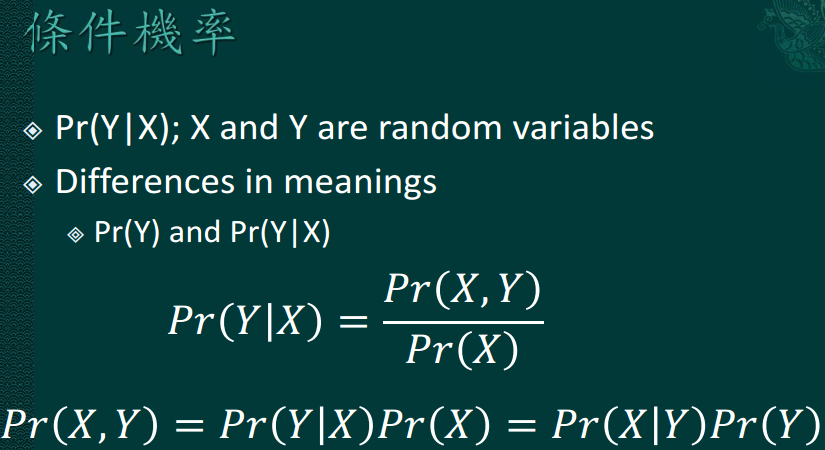
\includegraphics{prob-corelation.png}
\caption{prob-corelation}
\end{figure}

\begin{itemize}
\tightlist
\item
  假定Pr(C)=0.1,Pr(fever)=0.2,一個發燒病人得到肺炎的機率Pr(C\textbar fever)是多少?

  \begin{itemize}
  \tightlist
  \item
    計算Pr(C\textbar fever)/Pr(C)。這一個比例增加多少倍?
  \end{itemize}
\end{itemize}

    \begin{tcolorbox}[breakable, size=fbox, boxrule=1pt, pad at break*=1mm,colback=cellbackground, colframe=cellborder]
\prompt{In}{incolor}{3}{\boxspacing}
\begin{Verbatim}[commandchars=\\\{\}]
\PY{p}{;}\PY{p}{;} \PY{n}{A}
\PY{p}{(}\PY{n}{define} \PY{n}{pr}\PY{p}{:}\PY{n}{C} \PY{l+m+mf}{0.1}\PY{p}{)}  \PY{p}{;}\PY{p}{;} \PY{n}{Pr}\PY{p}{(}\PY{n}{C}\PY{p}{)}
\PY{p}{(}\PY{n}{define} \PY{n}{pr}\PY{p}{:}\PY{n}{fever} \PY{l+m+mf}{0.2}\PY{p}{)}  \PY{p}{;}\PY{p}{;} \PY{n}{Pr}\PY{p}{(}\PY{n}{fever}\PY{p}{)}
\PY{p}{(}\PY{n}{define} \PY{n}{pr}\PY{p}{:}\PY{n}{fever}\PY{n+nd}{@C} \PY{l+m+mf}{0.879}\PY{p}{)}  \PY{p}{;}\PY{p}{;} \PY{n}{Pr}\PY{p}{(}\PY{n}{fever}\PY{o}{|}\PY{n}{C}\PY{p}{)}

\PY{p}{(}\PY{n}{define} \PY{n}{pr}\PY{p}{:}\PY{n}{fever}\PY{o}{\PYZam{}}\PY{n}{C} \PY{p}{(}\PY{o}{*} \PY{n}{pr}\PY{p}{:}\PY{n}{fever}\PY{n+nd}{@C} \PY{n}{pr}\PY{p}{:}\PY{n}{C}\PY{p}{)}\PY{p}{)}  \PY{p}{;}\PY{p}{;} \PY{n}{Pr}\PY{p}{(}\PY{n}{fever}\PY{p}{,} \PY{n}{C}\PY{p}{)}
\PY{p}{(}\PY{n}{define} \PY{n}{pr}\PY{p}{:}\PY{n}{C}\PY{n+nd}{@fever} \PY{p}{(}\PY{o}{/} \PY{n}{pr}\PY{p}{:}\PY{n}{fever}\PY{o}{\PYZam{}}\PY{n}{C} \PY{n}{pr}\PY{p}{:}\PY{n}{fever}\PY{p}{)}\PY{p}{)}  \PY{p}{;}\PY{p}{;} \PY{n}{Pr}\PY{p}{(}\PY{n}{C}\PY{o}{|}\PY{n}{fever}\PY{p}{)} \PY{o}{=} \PY{n}{Pr}\PY{p}{(}\PY{n}{fever}\PY{p}{,} \PY{n}{C}\PY{p}{)} \PY{o}{/} \PY{n}{Pr}\PY{p}{(}\PY{n}{fever}\PY{p}{)}

\PY{p}{(}\PY{n}{displayln} \PY{p}{(}\PY{n}{string}\PY{o}{\PYZhy{}}\PY{n}{append} \PY{l+s+s2}{\PYZdq{}}\PY{l+s+s2}{* Pr(fever|C) 是 }\PY{l+s+s2}{\PYZdq{}} \PY{p}{(}\PY{n}{number}\PY{o}{\PYZhy{}}\PY{o}{\PYZgt{}}\PY{n}{string} \PY{n}{pr}\PY{p}{:}\PY{n}{C}\PY{n+nd}{@fever}\PY{p}{)}\PY{p}{)}\PY{p}{)}
\PY{p}{(}\PY{n}{displayln} \PY{p}{(}\PY{n}{string}\PY{o}{\PYZhy{}}\PY{n}{append} \PY{l+s+s2}{\PYZdq{}}\PY{l+s+s2}{  \PYZhy{} Pr(C|fever) / Pr(C) 是 }\PY{l+s+s2}{\PYZdq{}} \PY{p}{(}\PY{n}{number}\PY{o}{\PYZhy{}}\PY{o}{\PYZgt{}}\PY{n}{string} \PY{p}{(}\PY{o}{/} \PY{n}{pr}\PY{p}{:}\PY{n}{C}\PY{n+nd}{@fever} \PY{n}{pr}\PY{p}{:}\PY{n}{C}\PY{p}{)}\PY{p}{)} \PY{l+s+s2}{\PYZdq{}}\PY{l+s+s2}{ (倍)}\PY{l+s+s2}{\PYZdq{}}\PY{p}{)}\PY{p}{)}
\end{Verbatim}
\end{tcolorbox}

    \begin{Verbatim}[commandchars=\\\{\}]
* Pr(fever|C) 是 0.4395
  - Pr(C|fever) / Pr(C) 是 4.395 (倍)
    \end{Verbatim}

    \begin{itemize}
\tightlist
\item
  假定Pr(fever\textbar¬C)=0.01、Pr(C)=0.1,一個發燒病人得到肺炎的機率Pr(C\textbar fever)是多少?

  \begin{itemize}
  \tightlist
  \item
    Pr(C\textbar fever) 還是 Pr(¬C\textbar fever) 比較高?
  \end{itemize}
\end{itemize}

    \begin{tcolorbox}[breakable, size=fbox, boxrule=1pt, pad at break*=1mm,colback=cellbackground, colframe=cellborder]
\prompt{In}{incolor}{5}{\boxspacing}
\begin{Verbatim}[commandchars=\\\{\}]
\PY{p}{;}\PY{p}{;} \PY{n}{B}
\PY{p}{(}\PY{n}{define} \PY{n}{pr}\PY{p}{:}\PY{n}{C} \PY{l+m+mf}{0.1}\PY{p}{)}          \PY{p}{;}\PY{p}{;} \PY{n}{Pr}\PY{p}{(}\PY{n}{C}\PY{p}{)}
\PY{p}{(}\PY{n}{define} \PY{n}{pr}\PY{p}{:}\PY{err}{¬}\PY{n}{C} \PY{p}{(}\PY{o}{\PYZhy{}} \PY{l+m+mi}{1} \PY{n}{pr}\PY{p}{:}\PY{n}{C}\PY{p}{)}\PY{p}{)}  \PY{p}{;}\PY{p}{;} \PY{n}{Pr}\PY{p}{(}\PY{err}{¬}\PY{n}{C}\PY{p}{)}
\PY{p}{(}\PY{n}{define} \PY{n}{pr}\PY{p}{:}\PY{n}{fever} \PY{l+m+mf}{0.2}\PY{p}{)}

\PY{p}{(}\PY{n}{define} \PY{n}{pr}\PY{p}{:}\PY{n}{fever}\PY{n+nd}{@C} \PY{l+m+mf}{0.879}\PY{p}{)}  \PY{p}{;}\PY{p}{;} \PY{n}{Pr}\PY{p}{(}\PY{n}{fever}\PY{o}{|}\PY{n}{C}\PY{p}{)}
\PY{p}{(}\PY{n}{define} \PY{n}{pr}\PY{p}{:}\PY{n}{fever}\PY{o}{@}\PY{err}{¬}\PY{n}{C} \PY{l+m+mf}{0.01}\PY{p}{)}  \PY{p}{;}\PY{p}{;} \PY{n}{Pr}\PY{p}{(}\PY{n}{fever}\PY{o}{|}\PY{err}{¬}\PY{n}{C}\PY{p}{)}

\PY{p}{(}\PY{n}{define} \PY{n}{pr}\PY{p}{:}\PY{n}{fever}\PY{o}{\PYZam{}}\PY{err}{¬}\PY{n}{C} \PY{p}{(}\PY{o}{*} \PY{n}{pr}\PY{p}{:}\PY{n}{fever}\PY{o}{@}\PY{err}{¬}\PY{n}{C} \PY{n}{pr}\PY{p}{:}\PY{err}{¬}\PY{n}{C}\PY{p}{)}\PY{p}{)}
\PY{p}{(}\PY{n}{define} \PY{n}{pr}\PY{p}{:}\PY{err}{¬}\PY{n}{C}\PY{n+nd}{@fever} \PY{p}{(}\PY{o}{/} \PY{n}{pr}\PY{p}{:}\PY{n}{fever}\PY{o}{\PYZam{}}\PY{err}{¬}\PY{n}{C} \PY{n}{pr}\PY{p}{:}\PY{n}{fever}\PY{p}{)}\PY{p}{)}
\PY{p}{(}\PY{n}{define} \PY{n}{pr}\PY{p}{:}\PY{n}{C}\PY{n+nd}{@fever} \PY{p}{(}\PY{o}{\PYZhy{}} \PY{l+m+mi}{1} \PY{n}{pr}\PY{p}{:}\PY{err}{¬}\PY{n}{C}\PY{n+nd}{@fever}\PY{p}{)}\PY{p}{)}

\PY{p}{(}\PY{n}{displayln} \PY{p}{(}\PY{n}{string}\PY{o}{\PYZhy{}}\PY{n}{append} \PY{l+s+s2}{\PYZdq{}}\PY{l+s+s2}{* 發燒病人得到武漢肺炎 (C) 的機率是:}\PY{l+s+s2}{\PYZdq{}} \PY{p}{(}\PY{n}{number}\PY{o}{\PYZhy{}}\PY{o}{\PYZgt{}}\PY{n}{string} \PY{n}{pr}\PY{p}{:}\PY{n}{C}\PY{n+nd}{@fever}\PY{p}{)}\PY{p}{)}\PY{p}{)}
\PY{p}{(}\PY{n}{displayln} \PY{p}{(}\PY{n}{string}\PY{o}{\PYZhy{}}\PY{n}{append} \PY{l+s+s2}{\PYZdq{}}\PY{l+s+s2}{  \PYZhy{} 在此條件下,Pr(¬C|fever) 為 }\PY{l+s+s2}{\PYZdq{}} \PY{p}{(}\PY{n}{number}\PY{o}{\PYZhy{}}\PY{o}{\PYZgt{}}\PY{n}{string} \PY{n}{pr}\PY{p}{:}\PY{err}{¬}\PY{n}{C}\PY{n+nd}{@fever}\PY{p}{)}\PY{p}{)}\PY{p}{)}
\PY{p}{(}\PY{n}{displayln} \PY{l+s+s2}{\PYZdq{}}\PY{l+s+s2}{    故 Pr(C|fever) \PYZgt{} Pr(¬C|fever)}\PY{l+s+s2}{\PYZdq{}}\PY{p}{)}
\end{Verbatim}
\end{tcolorbox}

    \begin{Verbatim}[commandchars=\\\{\}]
* 發燒病人得到武漢肺炎 (C) 的機率是:0.955
  - 在此條件下,Pr(¬C|fever) 為 0.045000000000000005
    故 Pr(C|fever) > Pr(¬C|fever)
    \end{Verbatim}

    \hypertarget{ux6bd4ux8f03-bfs-ux548c-ids}{%
\subsection{2. 比較 BFS 和 IDS}\label{ux6bd4ux8f03-bfs-ux548c-ids}}

\begin{itemize}
\tightlist
\item
  參考 AIMA Fig. 3.12 和相關說明 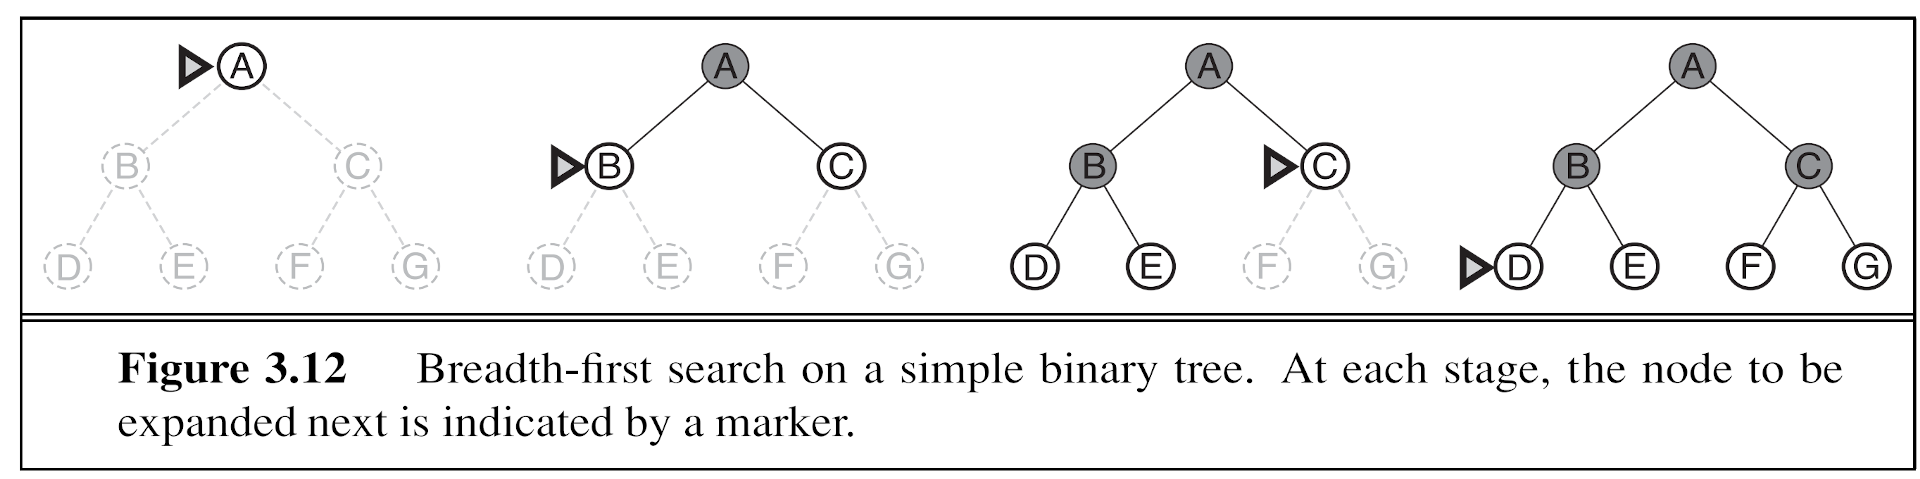
\includegraphics{aima-fig-3_12.png}

  \begin{itemize}
  \tightlist
  \item
    假定一個搜尋問題,每一個節點有兩個子節點
  \item
    利用BFS來搜尋答案的話,假定問題的答案在search tree
    的第三層(層數從零開始)的話,\textbf{最多} 需要進入 Fig. 3.7 graph
    search 演算法中的 loop do,做幾次的 choose?
  \end{itemize}
\end{itemize}

    \begin{tcolorbox}[breakable, size=fbox, boxrule=1pt, pad at break*=1mm,colback=cellbackground, colframe=cellborder]
\prompt{In}{incolor}{6}{\boxspacing}
\begin{Verbatim}[commandchars=\\\{\}]
\PY{k+kn}{from} \PY{n+nn}{collections} \PY{k+kn}{import} \PY{n}{namedtuple}

\PY{n}{Node} \PY{o}{=} \PY{n}{namedtuple}\PY{p}{(}\PY{l+s+s1}{\PYZsq{}}\PY{l+s+s1}{Node}\PY{l+s+s1}{\PYZsq{}}\PY{p}{,} \PY{p}{[}\PY{l+s+s1}{\PYZsq{}}\PY{l+s+s1}{name}\PY{l+s+s1}{\PYZsq{}}\PY{p}{,} \PY{l+s+s1}{\PYZsq{}}\PY{l+s+s1}{children}\PY{l+s+s1}{\PYZsq{}}\PY{p}{]}\PY{p}{)}
\PY{n}{Path} \PY{o}{=} \PY{n}{namedtuple}\PY{p}{(}\PY{l+s+s1}{\PYZsq{}}\PY{l+s+s1}{Path}\PY{l+s+s1}{\PYZsq{}}\PY{p}{,} \PY{p}{[}\PY{l+s+s1}{\PYZsq{}}\PY{l+s+s1}{nodes}\PY{l+s+s1}{\PYZsq{}}\PY{p}{,} \PY{l+s+s1}{\PYZsq{}}\PY{l+s+s1}{size}\PY{l+s+s1}{\PYZsq{}}\PY{p}{]}\PY{p}{)}

\PY{n}{NULL} \PY{o}{=} \PY{n}{Node}\PY{p}{(}\PY{l+s+s1}{\PYZsq{}}\PY{l+s+s1}{\PYZsq{}}\PY{p}{,} \PY{p}{[}\PY{p}{]}\PY{p}{)}

\PY{k}{def} \PY{n+nf}{build\PYZus{}node}\PY{p}{(}\PY{k+kp}{name}\PY{p}{)}\PY{p}{:}
    \PY{n}{node} \PY{o}{=} \PY{n}{Node}\PY{p}{(}\PY{k+kp}{name}\PY{p}{,} \PY{p}{[}\PY{p}{]}\PY{p}{)}
    \PY{k}{return} \PY{n}{node}


\PY{k}{def} \PY{n+nf}{build\PYZus{}nodes}\PY{p}{(}\PY{p}{)}\PY{p}{:}
    \PY{n}{cities} \PY{o}{=} \PY{p}{[}\PY{l+s+s1}{\PYZsq{}}\PY{l+s+s1}{A}\PY{l+s+s1}{\PYZsq{}}\PY{p}{,} \PY{l+s+s1}{\PYZsq{}}\PY{l+s+s1}{B}\PY{l+s+s1}{\PYZsq{}}\PY{p}{,} \PY{l+s+s1}{\PYZsq{}}\PY{l+s+s1}{C}\PY{l+s+s1}{\PYZsq{}}\PY{p}{,} \PY{l+s+s1}{\PYZsq{}}\PY{l+s+s1}{D}\PY{l+s+s1}{\PYZsq{}}\PY{p}{,} \PY{l+s+s1}{\PYZsq{}}\PY{l+s+s1}{E}\PY{l+s+s1}{\PYZsq{}}\PY{p}{,}
              \PY{l+s+s1}{\PYZsq{}}\PY{l+s+s1}{F}\PY{l+s+s1}{\PYZsq{}}\PY{p}{,} \PY{l+s+s1}{\PYZsq{}}\PY{l+s+s1}{G}\PY{l+s+s1}{\PYZsq{}}\PY{p}{,} \PY{l+s+s1}{\PYZsq{}}\PY{l+s+s1}{H}\PY{l+s+s1}{\PYZsq{}}\PY{p}{,} \PY{l+s+s1}{\PYZsq{}}\PY{l+s+s1}{I}\PY{l+s+s1}{\PYZsq{}}\PY{p}{,} \PY{l+s+s1}{\PYZsq{}}\PY{l+s+s1}{J}\PY{l+s+s1}{\PYZsq{}}\PY{p}{,}
              \PY{l+s+s1}{\PYZsq{}}\PY{l+s+s1}{K}\PY{l+s+s1}{\PYZsq{}}\PY{p}{,} \PY{l+s+s1}{\PYZsq{}}\PY{l+s+s1}{L}\PY{l+s+s1}{\PYZsq{}}\PY{p}{,} \PY{l+s+s1}{\PYZsq{}}\PY{l+s+s1}{M}\PY{l+s+s1}{\PYZsq{}}\PY{p}{,} \PY{l+s+s1}{\PYZsq{}}\PY{l+s+s1}{N}\PY{l+s+s1}{\PYZsq{}}\PY{p}{,} \PY{l+s+s1}{\PYZsq{}}\PY{l+s+s1}{O}\PY{l+s+s1}{\PYZsq{}}\PY{p}{]}
    \PY{k}{return} \PY{p}{\PYZob{}}\PY{n}{city}\PY{p}{:} \PY{n}{build\PYZus{}node}\PY{p}{(}\PY{n}{city}\PY{p}{)} \PY{k}{for} \PY{n}{city} \PY{o+ow}{in} \PY{n}{cities}\PY{p}{\PYZcb{}}

        
\PY{k}{def} \PY{n+nf}{link\PYZus{}nodes}\PY{p}{(}\PY{k+kp}{nodes}\PY{p}{,} \PY{n}{start}\PY{p}{,} \PY{o}{*}\PY{n}{ends}\PY{p}{)}\PY{p}{:}
    \PY{n}{start\PYZus{}node} \PY{o}{=} \PY{k+kp}{nodes}\PY{p}{[}\PY{n}{start}\PY{p}{]}
    \PY{k}{for} \PY{n}{end} \PY{o+ow}{in} \PY{n}{ends}\PY{p}{:}
        \PY{n}{start\PYZus{}node}\PY{o}{.}\PY{n}{children}\PY{o}{.}\PY{n}{append}\PY{p}{(}\PY{k+kp}{nodes}\PY{p}{[}\PY{n}{end}\PY{p}{]}\PY{p}{)}

\PY{k}{def} \PY{n+nf}{build\PYZus{}bfs\PYZus{}map}\PY{p}{(}\PY{p}{)}\PY{p}{:}
    \PY{k+kp}{nodes} \PY{o}{=} \PY{n}{build\PYZus{}nodes}\PY{p}{(}\PY{p}{)}
    
    \PY{n}{link\PYZus{}nodes}\PY{p}{(}\PY{k+kp}{nodes}\PY{p}{,} \PY{l+s+s1}{\PYZsq{}}\PY{l+s+s1}{A}\PY{l+s+s1}{\PYZsq{}}\PY{p}{,} \PY{l+s+s1}{\PYZsq{}}\PY{l+s+s1}{B}\PY{l+s+s1}{\PYZsq{}}\PY{p}{,} \PY{l+s+s1}{\PYZsq{}}\PY{l+s+s1}{C}\PY{l+s+s1}{\PYZsq{}}\PY{p}{)}
    \PY{n}{link\PYZus{}nodes}\PY{p}{(}\PY{k+kp}{nodes}\PY{p}{,} \PY{l+s+s1}{\PYZsq{}}\PY{l+s+s1}{B}\PY{l+s+s1}{\PYZsq{}}\PY{p}{,} \PY{l+s+s1}{\PYZsq{}}\PY{l+s+s1}{D}\PY{l+s+s1}{\PYZsq{}}\PY{p}{,} \PY{l+s+s1}{\PYZsq{}}\PY{l+s+s1}{E}\PY{l+s+s1}{\PYZsq{}}\PY{p}{)}
    \PY{n}{link\PYZus{}nodes}\PY{p}{(}\PY{k+kp}{nodes}\PY{p}{,} \PY{l+s+s1}{\PYZsq{}}\PY{l+s+s1}{C}\PY{l+s+s1}{\PYZsq{}}\PY{p}{,} \PY{l+s+s1}{\PYZsq{}}\PY{l+s+s1}{F}\PY{l+s+s1}{\PYZsq{}}\PY{p}{,} \PY{l+s+s1}{\PYZsq{}}\PY{l+s+s1}{G}\PY{l+s+s1}{\PYZsq{}}\PY{p}{)}
    \PY{n}{link\PYZus{}nodes}\PY{p}{(}\PY{k+kp}{nodes}\PY{p}{,} \PY{l+s+s1}{\PYZsq{}}\PY{l+s+s1}{D}\PY{l+s+s1}{\PYZsq{}}\PY{p}{,} \PY{l+s+s1}{\PYZsq{}}\PY{l+s+s1}{H}\PY{l+s+s1}{\PYZsq{}}\PY{p}{,} \PY{l+s+s1}{\PYZsq{}}\PY{l+s+s1}{I}\PY{l+s+s1}{\PYZsq{}}\PY{p}{)}
    \PY{n}{link\PYZus{}nodes}\PY{p}{(}\PY{k+kp}{nodes}\PY{p}{,} \PY{l+s+s1}{\PYZsq{}}\PY{l+s+s1}{E}\PY{l+s+s1}{\PYZsq{}}\PY{p}{,} \PY{l+s+s1}{\PYZsq{}}\PY{l+s+s1}{J}\PY{l+s+s1}{\PYZsq{}}\PY{p}{,} \PY{l+s+s1}{\PYZsq{}}\PY{l+s+s1}{K}\PY{l+s+s1}{\PYZsq{}}\PY{p}{)}
    \PY{n}{link\PYZus{}nodes}\PY{p}{(}\PY{k+kp}{nodes}\PY{p}{,} \PY{l+s+s1}{\PYZsq{}}\PY{l+s+s1}{F}\PY{l+s+s1}{\PYZsq{}}\PY{p}{,} \PY{l+s+s1}{\PYZsq{}}\PY{l+s+s1}{L}\PY{l+s+s1}{\PYZsq{}}\PY{p}{,} \PY{l+s+s1}{\PYZsq{}}\PY{l+s+s1}{M}\PY{l+s+s1}{\PYZsq{}}\PY{p}{)}
    \PY{n}{link\PYZus{}nodes}\PY{p}{(}\PY{k+kp}{nodes}\PY{p}{,} \PY{l+s+s1}{\PYZsq{}}\PY{l+s+s1}{G}\PY{l+s+s1}{\PYZsq{}}\PY{p}{,} \PY{l+s+s1}{\PYZsq{}}\PY{l+s+s1}{N}\PY{l+s+s1}{\PYZsq{}}\PY{p}{,} \PY{l+s+s1}{\PYZsq{}}\PY{l+s+s1}{O}\PY{l+s+s1}{\PYZsq{}}\PY{p}{)}
    
    \PY{k}{return} \PY{k+kp}{nodes}\PY{p}{[}\PY{l+s+s1}{\PYZsq{}}\PY{l+s+s1}{A}\PY{l+s+s1}{\PYZsq{}}\PY{p}{]}


\PY{k}{def} \PY{n+nf}{valid\PYZus{}path}\PY{p}{(}\PY{n}{path}\PY{p}{,} \PY{n}{start\PYZus{}name}\PY{p}{,} \PY{n}{end\PYZus{}name}\PY{p}{)}\PY{p}{:}
    \PY{n}{start} \PY{o}{=} \PY{n}{path}\PY{o}{.}\PY{k+kp}{nodes}\PY{p}{[}\PY{l+m+mi}{0}\PY{p}{]}
    \PY{n}{end} \PY{o}{=} \PY{n}{path}\PY{o}{.}\PY{k+kp}{nodes}\PY{p}{[}\PY{o}{\PYZhy{}}\PY{l+m+mi}{1}\PY{p}{]}

    \PY{k}{return} \PY{n}{start}\PY{o}{.}\PY{k+kp}{name} \PY{o}{==} \PY{n}{start\PYZus{}name} \PY{o+ow}{and} \PY{n}{end}\PY{o}{.}\PY{k+kp}{name} \PY{o}{==} \PY{n}{end\PYZus{}name}


\PY{k}{def} \PY{n+nf}{extend\PYZus{}path}\PY{p}{(}\PY{n}{path}\PY{p}{)}\PY{p}{:}
    \PY{n}{paths} \PY{o}{=} \PY{p}{[}\PY{p}{]}
    
    \PY{n}{path\PYZus{}nodes} \PY{o}{=} \PY{n}{path}\PY{o}{.}\PY{k+kp}{nodes}
    \PY{n}{start} \PY{o}{=} \PY{n}{path\PYZus{}nodes}\PY{p}{[}\PY{l+m+mi}{0}\PY{p}{]}
    \PY{n}{end} \PY{o}{=} \PY{n}{path\PYZus{}nodes}\PY{p}{[}\PY{o}{\PYZhy{}}\PY{l+m+mi}{1}\PY{p}{]}
    \PY{n}{children\PYZus{}of\PYZus{}end} \PY{o}{=} \PY{n}{end}\PY{o}{.}\PY{n}{children}

    \PY{n}{size} \PY{o}{=} \PY{n}{path}\PY{o}{.}\PY{n}{size}
    
    \PY{k}{for} \PY{n}{child} \PY{o+ow}{in} \PY{n}{children\PYZus{}of\PYZus{}end}\PY{p}{:}
        \PY{n}{new\PYZus{}nodes} \PY{o}{=} \PY{n}{path\PYZus{}nodes}\PY{o}{.}\PY{n}{copy}\PY{p}{(}\PY{p}{)}
        \PY{n}{new\PYZus{}nodes}\PY{o}{.}\PY{n}{append}\PY{p}{(}\PY{n}{child}\PY{p}{)}
        \PY{n}{paths}\PY{o}{.}\PY{n}{append}\PY{p}{(}\PY{n}{Path}\PY{p}{(}\PY{n}{new\PYZus{}nodes}\PY{p}{,} \PY{n}{size} \PY{o}{+} \PY{l+m+mi}{1}\PY{p}{)}\PY{p}{)}
        
    \PY{k}{return} \PY{n}{paths}


\PY{k}{def} \PY{n+nf}{bfs}\PY{p}{(}\PY{n}{frontier}\PY{p}{,} \PY{n}{es}\PY{p}{,} \PY{n}{times}\PY{p}{)}\PY{p}{:}
    \PY{k}{if} \PY{n+nb}{len}\PY{p}{(}\PY{n}{frontier}\PY{p}{)} \PY{o}{==} \PY{l+m+mi}{0} \PY{o+ow}{or} \PY{n}{frontier} \PY{o+ow}{is} \PY{k+kc}{None}\PY{p}{:}
        \PY{k}{raise} \PY{n+ne}{Exception}\PY{p}{(}\PY{p}{)}
    \PY{k}{else}\PY{p}{:}
        \PY{n}{path} \PY{o}{=} \PY{n}{frontier}\PY{o}{.}\PY{n}{pop}\PY{p}{(}\PY{l+m+mi}{0}\PY{p}{)}

        \PY{k}{if} \PY{n}{valid\PYZus{}path}\PY{p}{(}\PY{n}{path}\PY{p}{,} \PY{l+s+s1}{\PYZsq{}}\PY{l+s+s1}{A}\PY{l+s+s1}{\PYZsq{}}\PY{p}{,} \PY{l+s+s1}{\PYZsq{}}\PY{l+s+s1}{O}\PY{l+s+s1}{\PYZsq{}}\PY{p}{)}\PY{p}{:}
            \PY{k}{return} \PY{n}{path}\PY{p}{,} \PY{n}{times}
        \PY{k}{else}\PY{p}{:}
            \PY{n}{es}\PY{o}{.}\PY{n}{append}\PY{p}{(}\PY{n}{path}\PY{p}{)}
            \PY{n}{frontier}\PY{o}{.}\PY{n}{extend}\PY{p}{(}\PY{n}{extend\PYZus{}path}\PY{p}{(}\PY{n}{path}\PY{p}{)}\PY{p}{)}
            \PY{k}{return} \PY{n}{bfs}\PY{p}{(}\PY{n}{frontier}\PY{p}{,} \PY{n}{es}\PY{p}{,} \PY{n}{times} \PY{o}{+} \PY{l+m+mi}{1}\PY{p}{)}

\PY{n}{start} \PY{o}{=} \PY{n}{build\PYZus{}bfs\PYZus{}map}\PY{p}{(}\PY{p}{)}
\PY{n}{path}\PY{p}{,} \PY{n}{times} \PY{o}{=} \PY{n}{bfs}\PY{p}{(}\PY{p}{[}\PY{n}{Path}\PY{p}{(}\PY{p}{[}\PY{n}{start}\PY{p}{,} \PY{n}{start}\PY{p}{]}\PY{p}{,} \PY{l+m+mi}{0}\PY{p}{)}\PY{p}{]}\PY{p}{,} \PY{p}{[}\PY{p}{]}\PY{p}{,} \PY{l+m+mi}{0}\PY{p}{)}

\PY{n+nb}{print}\PY{p}{(}\PY{l+s+s1}{\PYZsq{}}\PY{l+s+s1}{A.}\PY{l+s+s1}{\PYZsq{}}\PY{p}{)}

\PY{n+nb}{print}\PY{p}{(}\PY{l+s+s1}{\PYZsq{}}\PY{l+s+s1}{BFS 路徑:}\PY{l+s+s1}{\PYZsq{}}\PY{p}{)}
\PY{k}{for} \PY{n}{node} \PY{o+ow}{in} \PY{n}{path}\PY{o}{.}\PY{k+kp}{nodes}\PY{p}{:}
    \PY{n+nb}{print}\PY{p}{(}\PY{n}{node}\PY{o}{.}\PY{k+kp}{name}\PY{p}{)}

\PY{n+nb}{print}\PY{p}{(}\PY{l+s+s2}{\PYZdq{}}\PY{l+s+s2}{最多需進入 loop 執行次數:}\PY{l+s+s2}{\PYZdq{}}\PY{p}{,} \PY{n}{times}\PY{p}{)}
\end{Verbatim}
\end{tcolorbox}

    \begin{Verbatim}[commandchars=\\\{\}]
A.
BFS 路徑:
A
A
C
G
O
最多需進入 loop 執行次數: 14
    \end{Verbatim}

    \begin{itemize}
\tightlist
\item
  參考 AIMA Fig. 3.18 和 Fig. 3.19 和相關說明和 p.~90 上的計算
  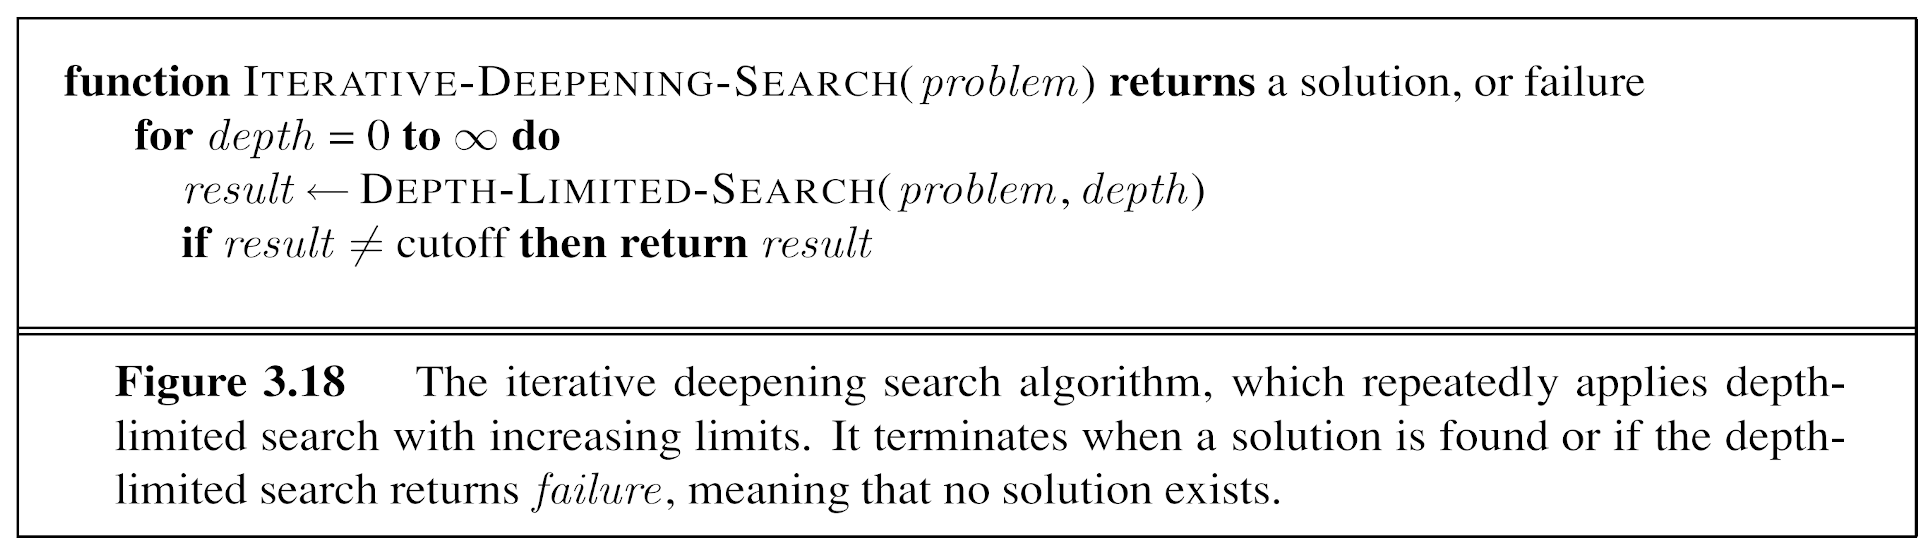
\includegraphics{aima-fig-3_18.png}
  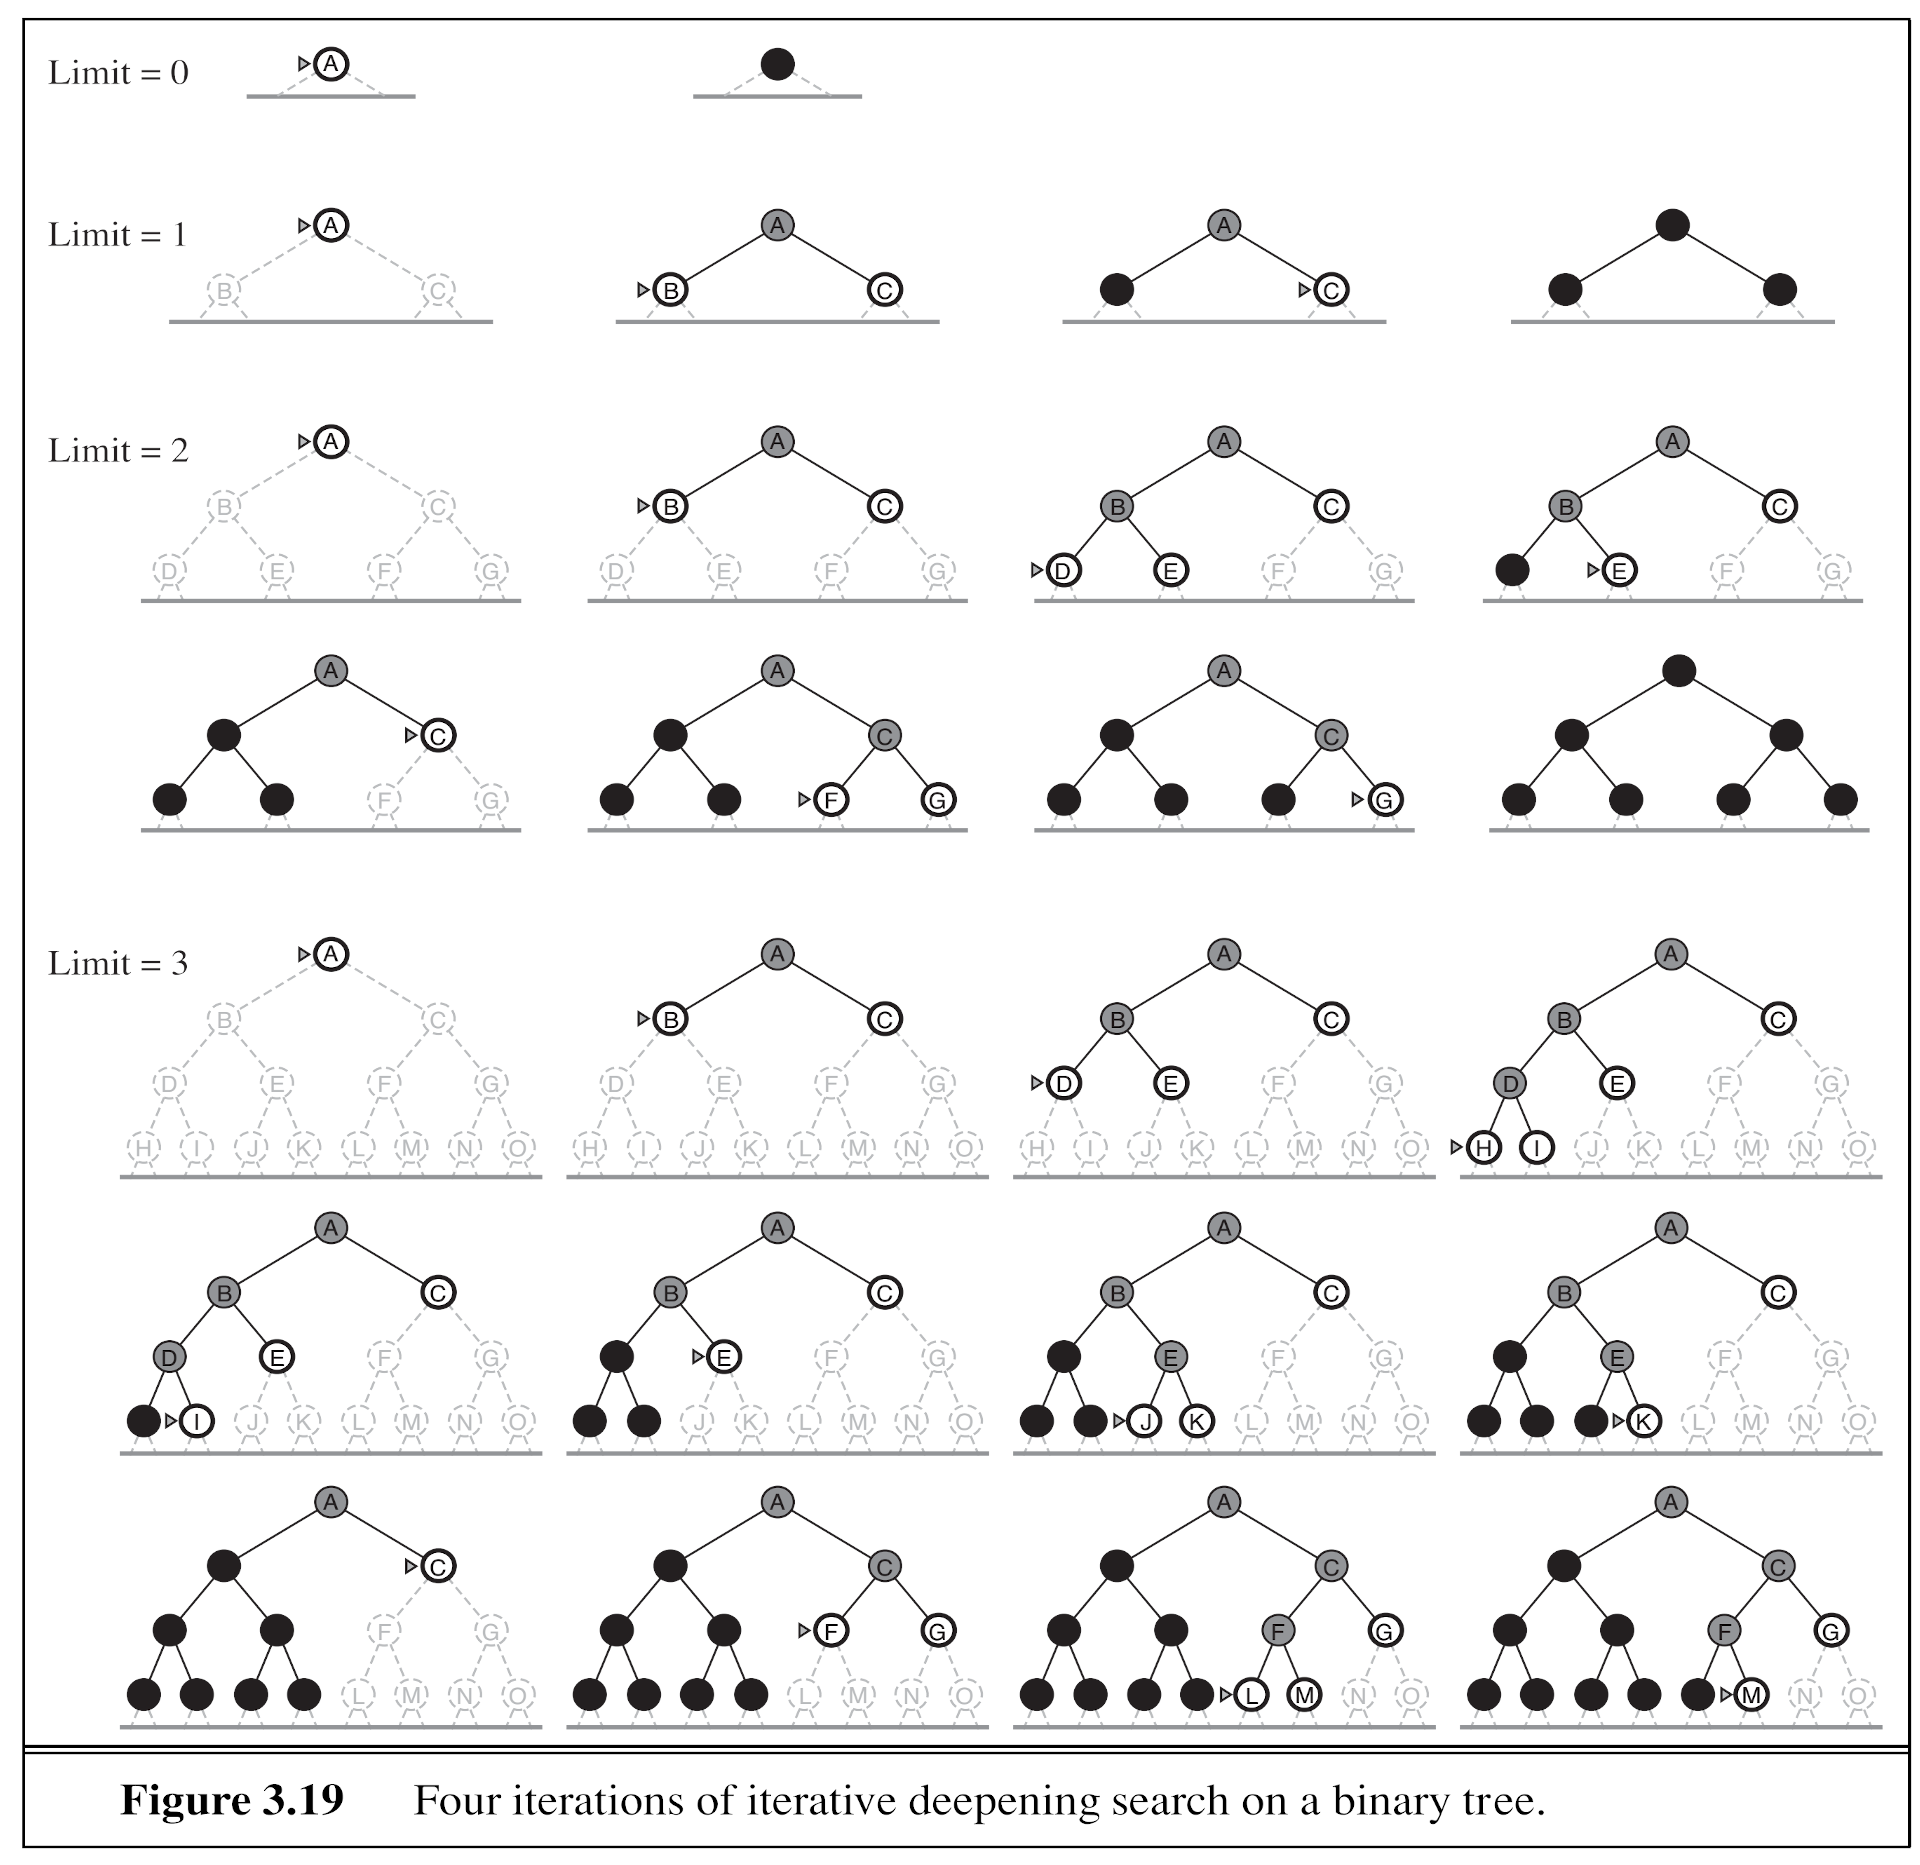
\includegraphics{aima-fig-3_19.png}
  
\includegraphics{aima-fun-ids.png}

  \begin{itemize}
  \tightlist
  \item
    假定一個搜尋問題,每一個節點有兩個子節點
  \item
    利用IDS來搜尋答案的話,假定問題的答案在search tree
    的第三層(層數從零開始)的話,\textbf{最多} 需要 choose
    多少節點才會找到答案?
  \end{itemize}
\end{itemize}

計算函式如下:

\[\sum_{n=0}^{n=d-1}(d-n)(b^{n+1})\]

    \begin{tcolorbox}[breakable, size=fbox, boxrule=1pt, pad at break*=1mm,colback=cellbackground, colframe=cellborder]
\prompt{In}{incolor}{13}{\boxspacing}
\begin{Verbatim}[commandchars=\\\{\}]
\PY{p}{(}\PY{n}{define} \PY{n}{depth} \PY{l+m+mi}{3}\PY{p}{)}
\PY{p}{(}\PY{n}{define} \PY{n}{branch} \PY{l+m+mi}{2}\PY{p}{)}

\PY{p}{(}\PY{n}{define} \PY{n}{loop}\PY{o}{\PYZhy{}}\PY{n}{count}
    \PY{p}{(}\PY{k}{lambda} \PY{p}{(}\PY{n}{d} \PY{n}{b} \PY{n}{n}\PY{p}{)}
        \PY{p}{(}\PY{k}{if} \PY{p}{(}\PY{o}{=} \PY{n}{n} \PY{l+m+mi}{0}\PY{p}{)}
            \PY{p}{(}\PY{o}{*} \PY{n}{d} \PY{n}{b}\PY{p}{)}
            \PY{p}{(}\PY{o}{+} \PY{p}{(}\PY{o}{*} \PY{p}{(}\PY{o}{\PYZhy{}} \PY{n}{d} \PY{n}{n}\PY{p}{)}
                  \PY{p}{(}\PY{n}{expt} \PY{n}{b} \PY{p}{(}\PY{o}{+} \PY{n}{n} \PY{l+m+mi}{1}\PY{p}{)}\PY{p}{)}\PY{p}{)}
               \PY{p}{(}\PY{n}{loop}\PY{o}{\PYZhy{}}\PY{n}{count} \PY{n}{d} \PY{n}{b} \PY{p}{(}\PY{o}{\PYZhy{}} \PY{n}{n} \PY{l+m+mi}{1}\PY{p}{)}\PY{p}{)}\PY{p}{)}\PY{p}{)}\PY{p}{)}\PY{p}{)}
               
\PY{p}{(}\PY{n}{define} \PY{n}{loops} \PY{p}{(}\PY{n}{loop}\PY{o}{\PYZhy{}}\PY{n}{count} \PY{p}{(}\PY{o}{+} \PY{n}{depth} \PY{l+m+mi}{1}\PY{p}{)} \PY{n}{branch} \PY{n}{depth}\PY{p}{)}\PY{p}{)}

\PY{p}{(}\PY{n}{displayln} \PY{p}{(}\PY{n}{string}\PY{o}{\PYZhy{}}\PY{n}{append} \PY{l+s+s2}{\PYZdq{}}\PY{l+s+s2}{* 最多會執行 }\PY{l+s+s2}{\PYZdq{}} \PY{p}{(}\PY{n}{number}\PY{o}{\PYZhy{}}\PY{o}{\PYZgt{}}\PY{n}{string} \PY{n}{loops}\PY{p}{)}  \PY{l+s+s2}{\PYZdq{}}\PY{l+s+s2}{ 次 loop}\PY{l+s+s2}{\PYZdq{}}\PY{p}{)}\PY{p}{)}
\end{Verbatim}
\end{tcolorbox}

    \begin{Verbatim}[commandchars=\\\{\}]
* 最多會執行 52 次 loop
    \end{Verbatim}

    \hypertarget{ux53c3ux7167-ai.ch3.dfs.bfs.pdf-ux7b2c29ux9801ux6295ux5f71ux7247ux4e0aux7684-8-puzzle-ux554fux984c}{%
\subsection{3. 參照 ai.ch3.dfs.bfs.pdf 第29頁投影片上的 8 puzzle
問題}\label{ux53c3ux7167-ai.ch3.dfs.bfs.pdf-ux7b2c29ux9801ux6295ux5f71ux7247ux4e0aux7684-8-puzzle-ux554fux984c}}

\begin{figure}
\centering
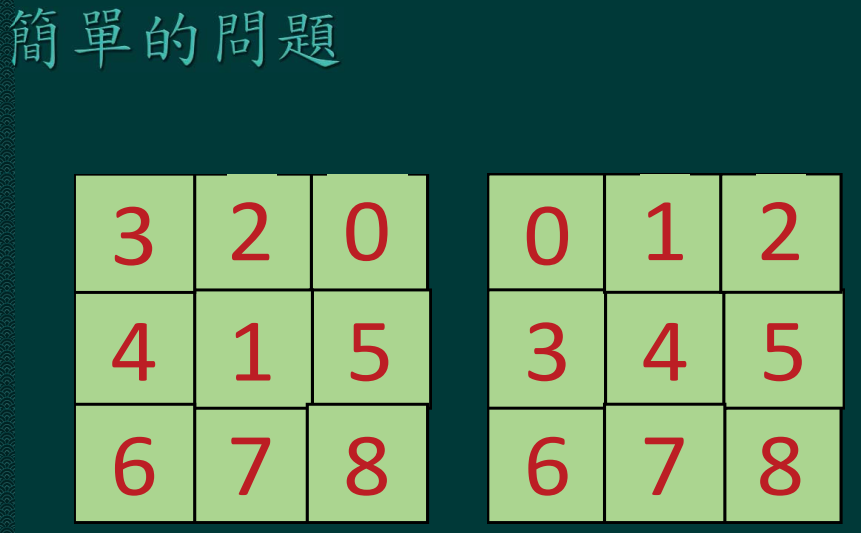
\includegraphics{slide-ch3-p29.png}
\caption{slide p29}
\end{figure}

\begin{itemize}
\tightlist
\item
  利用AIMA書本的 h1 和 h2 來找這一 8 puzzle 問題的答案
\item
  思考一下,如果使用 BFS 或者 DFS 的話,所需要 expand
  的節點的數目會不會多很多?
\end{itemize}

    \begin{tcolorbox}[breakable, size=fbox, boxrule=1pt, pad at break*=1mm,colback=cellbackground, colframe=cellborder]
\prompt{In}{incolor}{ }{\boxspacing}
\begin{Verbatim}[commandchars=\\\{\}]

\end{Verbatim}
\end{tcolorbox}


    % Add a bibliography block to the postdoc
    
    
    
\end{document}
